\documentclass[conference,a4paper]{IEEEtran}
\usepackage{amsmath,amssymb}
\usepackage{booktabs}
\usepackage{graphicx}
\usepackage{url}

\newcommand{\GapFormalMotorised}{0.061}
\newcommand{\RecallGapFormalMotorised}{0.081}
\newcommand{\NFormalMotorised}{2621}
\newcommand{\GapPedestrian}{0.094}
\newcommand{\RecallGapPedestrian}{0.119}
\newcommand{\NPedestrian}{2509}
\newcommand{\GapInformalMotorised}{0.197}
\newcommand{\RecallGapInformalMotorised}{0.263}
\newcommand{\NInformalMotorised}{1796}
\newcommand{\GapNonMotorised}{0.225}
\newcommand{\RecallGapNonMotorised}{0.277}
\newcommand{\NNonMotorised}{1026}
\newcommand{\ArAPgapCILo}{0.180}
\newcommand{\ArAPgapCIHi}{0.216}
\newcommand{\FormalMotorisedAPgapCILo}{0.043}
\newcommand{\FormalMotorisedAPgapCIHi}{0.081}
\newcommand{\PedestrianAPgapCILo}{0.073}
\newcommand{\PedestrianAPgapCIHi}{0.112}
\newcommand{\InformalMotorisedAPgapCILo}{0.180}
\newcommand{\InformalMotorisedAPgapCIHi}{0.217}
\newcommand{\NonMotorisedAPgapCILo}{0.195}
\newcommand{\NonMotorisedAPgapCIHi}{0.256}

\newcommand{\GapFormalMotorisedAltArch}{0.054}
\newcommand{\RecallGapFormalMotorisedAltArch}{0.065}
\newcommand{\GapPedestrianAltArch}{0.104}
\newcommand{\RecallGapPedestrianAltArch}{0.102}
\newcommand{\GapInformalMotorisedAltArch}{0.185}
\newcommand{\RecallGapInformalMotorisedAltArch}{0.267}
\newcommand{\GapNonMotorisedAltArch}{0.227}
\newcommand{\RecallGapNonMotorisedAltArch}{0.257}
\newcommand{\RobAGapAltArch}{+0.205}
\newcommand{\RobBGapAltArch}{+0.157}
\newcommand{\HeadlineMeanEOne}{0.385}
\newcommand{\HeadlineMeanETwo}{0.483}
\newcommand{\HeadlineMeanEOneAltArch}{0.426}
\newcommand{\HeadlineMeanETwoAltArch}{0.523}


% Anonymised for review; swap for the real GitHub URL at camera-ready.
\newcommand{\CodeLink}{\url{https://anonymous.4open.science/r/ecce2027-4E83}}

\begin{document}

\title{Class-Resolved Cross-City Transfer of YOLO Vehicle Detectors: A Dhaka-to-Chattogram Study}

% Blinded for initial review submission -- ECCE 2027 uses double-blind review;
% author name/affiliation/email are supplied separately in the submission
% system and must NOT appear in the PDF at initial submission. Restore the
% block below at camera-ready.
% \author{
% \IEEEauthorblockN{1\textsuperscript{st} MD. Mahi Islam}
% \IEEEauthorblockA{Dept.\ of CSE, CUET\\
% Chattogram, Bangladesh\\
% u2104054@student.cuet.ac.bd}
% }
\author{
\IEEEauthorblockN{Anonymous Author(s)}
\IEEEauthorblockA{Affiliation withheld for double-blind review}
}

\maketitle

\begin{abstract}
% Numbers below are pulled from paper/tables/macros*.tex, not hand-typed.
Object detectors trained on one Bangladeshi city's road imagery are known to lose
accuracy when deployed in another, and detectors trained on structured traffic are
known to transfer poorly to unstructured South Asian traffic. What is not established
is whether a same-city, same-protocol transfer gap is spread evenly across vehicle
types, or concentrated in specific ones. Holding annotation protocol and camera
viewpoint fixed, we train YOLOv8s detectors on Dhaka dash-camera imagery from the
BadODD dataset and evaluate them on a held-out Chattogram set, against a
Chattogram-trained reference, using a 3-fold temporal-block cross-validation design
plus two leave-one-corridor-out robustness folds. We find the transfer gap is not
uniform: it is smallest for globally-standard motorised classes (car, bus, truck,
motorbike; AP50 gap \GapFormalMotorised) and 3--4$\times$ larger
for two locally-specific informal and non-motorised modes -- CNG/battery
auto-rickshaws (AP50 gap \GapInformalMotorised) and cycle-rickshaws (AP50 gap
\GapNonMotorised) -- with an even larger gap in recall, the operating point that
determines whether a vehicle is counted at all. The pattern replicates in both
robustness folds and under a second, newer detector architecture (YOLO26s). Because vehicle counts derived from such detectors feed
downstream traffic-signal timing, this class-concentrated blind spot has a
direct equity implication we discuss.
\end{abstract}

\begin{IEEEkeywords}
object detection, domain transfer, heterogeneous traffic, Bangladesh, YOLO
\end{IEEEkeywords}

\section{Introduction}
\label{sec:intro}
% One claim per paragraph; paraphrase, never copy source sentences.

Urban traffic in Bangladeshi cities is a heterogeneous, largely non-lane-based mix,
with informal and non-motorised vehicles sharing the carriageway alongside cars, buses
and trucks -- a mix that differs sharply from the structured traffic most detection
benchmarks are built on.
Large driving-scene benchmarks such as BDD100K \cite{yu2020bdd100k} and the original
COCO object-detection benchmark \cite{lin2014coco} -- the source of the AP50 metric
and evaluation protocol we use throughout this paper -- are drawn overwhelmingly from
structured, lane-based traffic and do not include informal-transport classes at all.
Object detectors intended to feed automated traffic monitoring or signal control must
therefore work well on exactly the vehicle types structured-traffic benchmarks
under-represent.

Two facts are already established in the literature and are not this paper's
contribution. First, detectors trained on structured traffic transfer poorly to
unstructured, developing-city traffic: fixed-camera evaluation on BMD-45 reports a 2.5x
mAP gap between a structured-traffic-trained detector and an in-domain one on an
expert-annotated reference set \cite{sharma2026bmd45}; the gap is smaller but still
consistently positive ($\approx$1.1x mAP@0.5:0.95) in that paper's main
architecture-matched cross-dataset benchmark table for a comparably-sized YOLO variant,
so the size of a structured-to-unstructured gap is itself evaluation-protocol-dependent.
Second, cross-city detection generalisation is an active,
separately benchmarked problem, evidenced by ongoing challenge tracks
\cite{aicitychallenge2026} and multi-task cross-city benchmarks such as
CityTransfer-Bench \cite{qian2026citygen}. Neither source reports whether a same-city,
same-annotation-protocol transfer gap concentrates on specific vehicle classes.

This paper isolates that question. Using BadODD \cite{baig2024badodd}, a single
dashcam dataset annotated under one protocol across nine Bangladeshi districts
including both Dhaka and Chattogram, we hold camera viewpoint and annotation protocol
fixed and ask whether a detector trained on Dhaka imagery, once evaluated on
Chattogram imagery, shows a performance drop that is uniform across vehicle classes or
instead concentrated in specific modes -- particularly the informal and non-motorised ones
that existing structured-traffic benchmarks do not cover at all? We report recall
(whether a vehicle is detected at all) as the primary quantity of interest, since a
missed vehicle is what would later bias a classified count in a downstream
traffic-monitoring pipeline.

Our contribution is a controlled, class-resolved measurement of this gap, not a new
detector or dataset. We find the gap is $3$--$4\times$ larger for two locally-specific
modes -- CNG/battery auto-rickshaws and cycle-rickshaws -- than for globally-standard
motorised classes, and that this pattern is robust both to the cross-validation design
used to measure it and to the choice of detector architecture.

\section{Related Work}
\label{sec:related}

BadODD \cite{baig2024badodd} is the dataset this paper builds on; its class taxonomy,
defined by power source and size rather than local vehicle name, is what makes a
same-protocol Dhaka-Chattogram comparison possible in the first place (Section
\ref{sec:dataset}).

BMD-45 \cite{sharma2026bmd45} establishes that a structured-to-unstructured camera
domain gap exists, attributing it to viewpoint and elevation differences between
structured and CCTV-style fixed cameras. That is a different axis from the one studied
here: BadODD is dash-mounted in both cities, so our comparison holds viewpoint fixed
and isolates city/location effects instead. BMD-45's benchmark tables do not report a
class-wise breakdown of its transfer gap, so whether that gap is itself
class-concentrated is, to our knowledge, still open. Other South Asian unstructured-traffic
datasets such as IDD \cite{varma2019idd} cover a broader mix of road users but are
single-region collections and do not offer the same-protocol multi-city split that
lets us hold annotation protocol fixed while varying city, the way BadODD does.

Bangladeshi-vehicle YOLO benchmarks, e.g.\ \cite{hossain2025yolobd}, confirm YOLO
variants have already been evaluated extensively on Bangladeshi road imagery and that
rare classes collapse under class imbalance -- consistent with what we observe for
under-30-instance classes in Section \ref{sec:results}. Rare-class collapse under
long-tailed label distributions is itself a well-studied general problem in object
detection \cite{lin2017focalloss,li2022eqfl}, but that line of work targets a fixed
in-domain class imbalance; we study a case where class imbalance interacts with a
cross-city domain shift, and neither \cite{hossain2025yolobd} nor the general
long-tail literature performs a cross-city or cross-domain transfer evaluation.

Detection bias against vulnerable road users is a recognised problem in the wider
perception literature \cite{katare2024bias,wilson2019predictive}, studied there on
structured-traffic data (nuScenes, BDD100K) and framed around demographic or safety
disparities among pedestrians. Our framing differs: the downstream harm we are
concerned with is a counting/allocation one (Section \ref{sec:discussion}), the
disparity is across vehicle \emph{class} rather than pedestrian demographic group, and
the setting is unstructured, non-lane-based traffic rather than structured urban
driving.

CityTransfer-Bench \cite{qian2026citygen} benchmarks cross-city generalisation broadly
across perception, segmentation and planning, and proposes closing the gap via
synthetic target-city imagery. It is not class-resolved and does not target
Bangladeshi informal transport modes specifically.

More broadly, the Dhaka-to-Chattogram gap we measure is an instance of the domain-shift
problem surveyed in \cite{wang2018domainadapt}: a model trained on a source
distribution (Dhaka) underperforming on a related but distinct target distribution
(Chattogram) without target-domain adaptation. We do not apply a domain-adaptation
method here -- our contribution is measuring where, class-wise, that gap is largest --
but the survey's taxonomy of feature-level vs.\ instance-level adaptation is a natural
starting point for closing the gap this paper documents; concrete instance-level
methods such as \cite{chen2018domainadaptivefrcnn} already adapt detectors across
exactly this kind of camera/viewpoint domain shift, but have not, to our knowledge,
been applied to a same-city class imbalance of the kind reported here.

\section{Dataset and Experimental Setup}
\label{sec:dataset}

\subsection{Dataset}
We use the Zenodo release of BadODD (DOI \texttt{10.5281/zenodo.13823687}, CC BY 4.0),
10{,}032 fully labelled dash-camera images across 9 Bangladeshi districts, 11 vehicle
classes with non-zero Chattogram or Dhaka instances (\texttt{train} and
\texttt{wheelchair} have zero Chattogram instances and are dropped). Classes are
defined by physical characteristic rather than local name -- notably,
\texttt{three\_wheeler} (paddle-powered, i.e.\ the cycle-rickshaw) is a distinct class
from \texttt{auto\_rickshaw} (gas/electric-powered, covering both CNG auto-rickshaws
and battery-powered "tomtom"/easy-bikes). Of the 11 trained classes, 7 have at least
30 Chattogram test instances and are reported individually (Table
\ref{tab:headline}); the remaining 4 (\texttt{bicycle}, \texttt{cart\_vehicle},
\texttt{priority\_vehicle}, \texttt{construction\_vehicle}) are below that threshold
and are reported only as part of mode-group aggregates, weighted by instance count so
they cannot dominate a group's number.

We group the 7 headline classes into 4 mode groups: \emph{pedestrian} (person),
\emph{non-motorised} (three-wheeler/cycle-rickshaw, plus the below-threshold bicycle
and cart vehicle), \emph{informal motorised} (auto-rickshaw), and \emph{formal
motorised} (car, bus, truck, motorbike, plus the below-threshold priority and
construction vehicles).

\subsection{Splits and cross-validation}
Chattogram's 3 continuous video drives are each split into 3 temporal blocks with a
$\geq$15-second buffer between blocks to avoid near-duplicate leakage, giving a
3-fold cross-validation design. Dhaka training sets are subsampled (seed 42) to match
each Chattogram fold's training-set size and day/night ratio, so that a
Dhaka-vs-Chattogram comparison is not confounded by training-set size. Two further
robustness folds hold out one entire daytime corridor each (no temporal-block cuts),
subsampled to the same training size, to check the main result is not an artifact of
the temporal-block partitioning. Full split counts are in \texttt{notes/splits.md}.

\subsection{Models and training}
YOLOv8s (Ultralytics 8.4.155), a single-stage detector in the YOLO lineage
that began with the original YOLO/YOLOv3 formulation \cite{redmon2018yolov3} and has
been reviewed in detail up to YOLOv8 by \cite{terven2023yolo}, COCO-pretrained, 640px
input, fixed hyperparameters and seed (42, deterministic) across every run, 100 epochs,
no early stopping, no model-selection on evaluation data (\texttt{last.pt} used
throughout). Two experiment families: E1 (Dhaka-trained, 3 folds) and E2
(Chattogram-trained, 3 folds), plus the 2 robustness-fold models. Every run exports raw
predictions at confidence 0.001 in COCO format, so all metrics below are recomputed
offline. All 8 runs are then repeated with YOLO26s \cite{jocher2026yolo26} (same
Ultralytics version, COCO-pretrained), with splits, seed and hyperparameters unchanged
-- including the SGD optimizer, rather than YOLO26's default MuSGD -- so that only the
model differs, to test whether the result depends on the architecture. Code, the
offline metric-recomputation pipeline and every prediction file behind the numbers
below are available at \CodeLink{}.

\begin{figure*}[t]
\centering
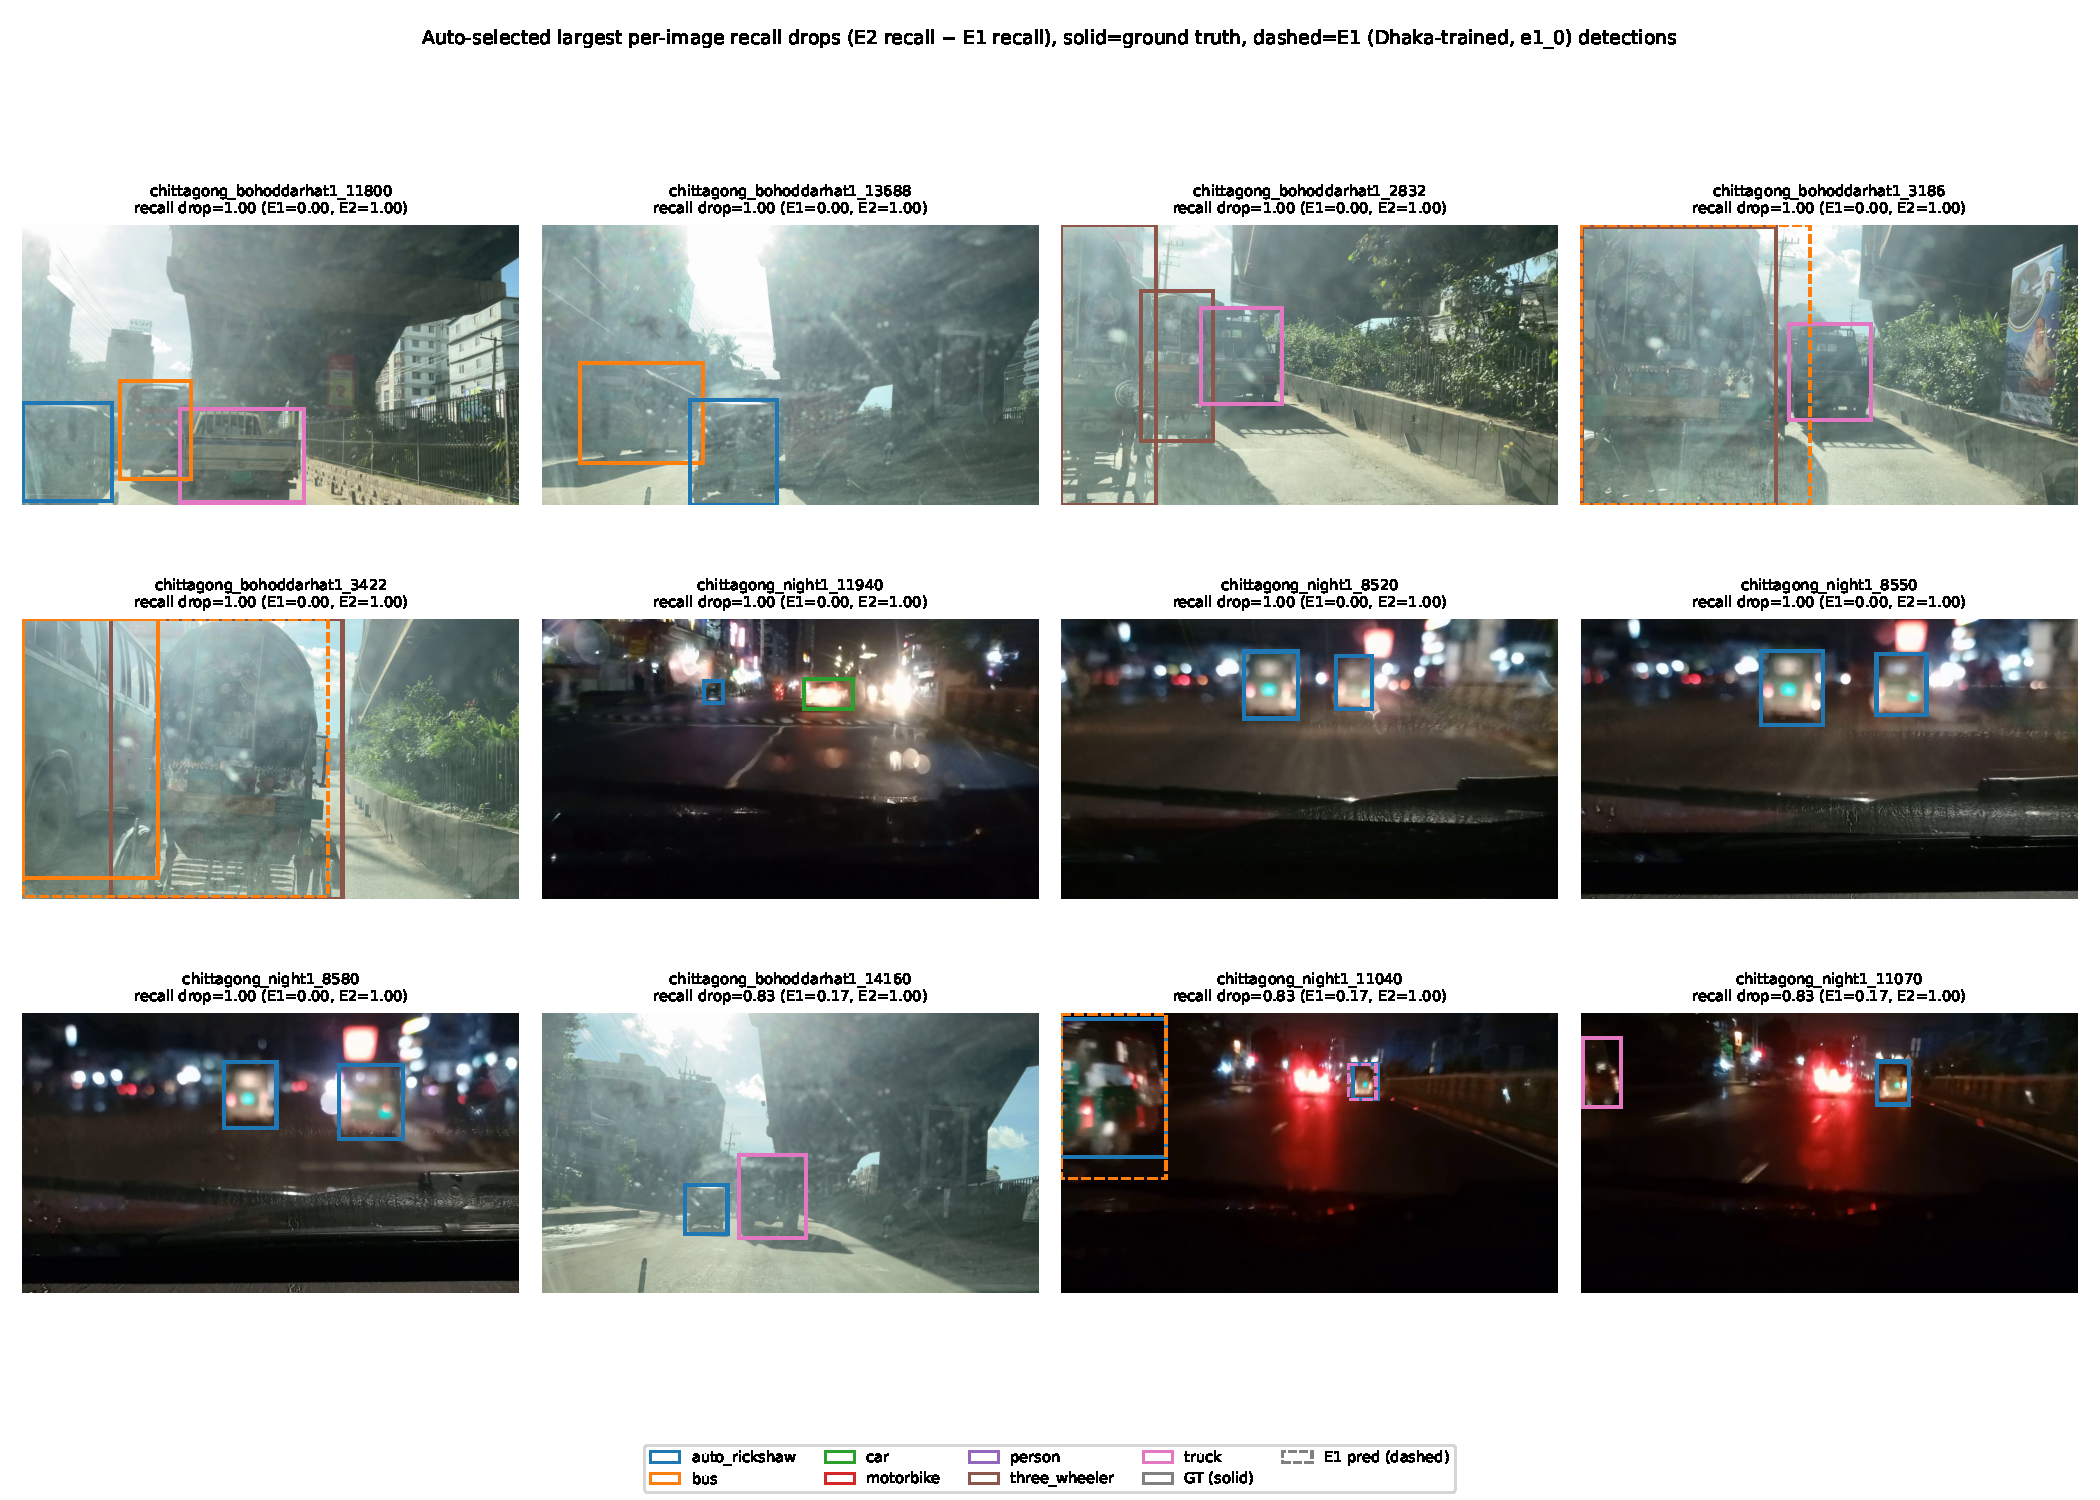
\includegraphics[width=0.95\linewidth]{figures/qualitative_failures.pdf}
\caption{The 12 \texttt{ctg\_pooled\_eval} images with the largest per-image recall
drop (E2 recall $-$ E1 recall, headline classes, $\geq$2 GT boxes), selected
automatically by \texttt{src/run\_wp4\_qualitative.py} -- not hand-picked. Solid boxes:
ground truth. Dashed boxes: E1 (\texttt{e1\_0}) detections above its operating
threshold. Most panels show E1 missing every GT box in the frame. Discussed alongside
the quantitative results in Section \ref{sec:results}.}
\label{fig:qualitative}
\end{figure*}

\subsection{Metrics}
Per-class AP50 (COCO-style, 101-point interpolation, following the original COCO
evaluation protocol \cite{lin2014coco}) and recall at a fixed operating
point, chosen per model by maximising pooled F1 over the 7 headline classes on that
model's own in-domain evaluation fold and held fixed for every other evaluation of
that model. 95\% confidence intervals are image-level bootstrap (resampling images
with replacement; local implementation validated against Kaggle's own pycocotools
output, exact match on the non-bootstrapped point estimate).

\section{Results}
\label{sec:results}

\begin{table}[t]
\centering
\caption{Dhaka-trained (E1, mean of 3 folds) vs.\ Chattogram-trained reference (E2, out-of-fold pooled), evaluated on the identical 1{,}121-image Chattogram test set. AP50 gap = E2 $-$ E1, with 95\% image-level bootstrap CI (300 resamples).}
\label{tab:headline}
\resizebox{\columnwidth}{!}{%
\begin{tabular}{lrrrl}
\toprule
Class & $n$ & E1 AP50 & E2 AP50 & AP50 gap [95\% CI] \\
\midrule
Auto-rickshaw & 1796 & 0.558 & 0.755 & +0.197 [+0.180, +0.216] \\
Bus & 411 & 0.308 & 0.325 & +0.017 [-0.035, +0.070] \\
Car & 1122 & 0.521 & 0.614 & +0.094 [+0.069, +0.117] \\
Motorbike & 401 & 0.414 & 0.369 & -0.045 [-0.096, +0.002] \\
Person & 2509 & 0.272 & 0.366 & +0.094 [+0.077, +0.111] \\
Three-wheeler (cycle-rick.) & 988 & 0.327 & 0.561 & +0.234 [+0.203, +0.267] \\
Truck & 668 & 0.295 & 0.393 & +0.098 [+0.056, +0.137] \\
\bottomrule
\end{tabular}%
}
\end{table}


Table \ref{tab:headline} compares E1 (mean of the 3 Dhaka-trained folds) against E2
(the 3 Chattogram-trained folds' out-of-fold pooled predictions), both evaluated on
the same 1{,}121-image Chattogram test set. Every headline class except
\texttt{motorbike} shows a positive AP50 gap (E2 above E1), but the size of that gap
varies by more than an order of magnitude across classes.

\begin{table}[t]
\centering
\caption{Transfer gap aggregated by mode group, weighted by each class's Chattogram instance count.}
\label{tab:modegroup}
\begin{tabular}{lrrrr}
\toprule
Mode group & $n$ & E1 AP50 & E2 AP50 & AP50 gap \\
\midrule
Formal motorised & 2621 & 0.410 & 0.471 & +0.061 \\
Pedestrian & 2509 & 0.272 & 0.366 & +0.094 \\
Informal motorised & 1796 & 0.558 & 0.755 & +0.197 \\
Non-motorised & 1026 & 0.315 & 0.540 & +0.225 \\
\bottomrule
\end{tabular}
\end{table}


Table \ref{tab:modegroup} aggregates by mode group, weighted by each class's
Chattogram instance count. The formal-motorised group -- car, bus, truck, motorbike,
the classes any general-purpose, COCO-trained detector would already recognise --
shows the smallest gap (\GapFormalMotorised{} AP50, \RecallGapFormalMotorised{}
recall). The two locally-specific groups show substantially larger gaps: informal
motorised (auto-rickshaw) at \GapInformalMotorised{} AP50 /
\RecallGapInformalMotorised{} recall, and non-motorised (cycle-rickshaw-dominated) at
\GapNonMotorised{} AP50 / \RecallGapNonMotorised{} recall -- both roughly $3$--$4\times$
the formal-motorised gap.

Per-class 95\% bootstrap CIs (Table \ref{tab:headline}) show this is not uniformly
noise: the \texttt{car}, \texttt{person}, \texttt{truck}, \texttt{three\_wheeler} and
\texttt{auto\_rickshaw} gaps all exclude zero, and the two largest gaps -- the two
locally-specific classes, auto-rickshaw [\ArAPgapCILo{}, \ArAPgapCIHi{}] and
three-wheeler -- are among the most clearly significant. Following the stated protocol
for a CI that spans zero, we report \texttt{bus} ($[-0.035,+0.070]$) and
\texttt{motorbike} ($[-0.096,+0.002]$) as \emph{no evidence of a class-level
difference} at this sample size, not as null findings for the formal-motorised group
as a whole -- the group's weighted point estimate is still driven upward by
\texttt{car} and \texttt{truck}, both individually significant.

\begin{table}[t]
\centering
\caption{Mode-group AP50 and recall transfer gaps with 95\% bootstrap CI (300 shared image resamples across all 11 classes).}
\label{tab:modegroupci}
\resizebox{\columnwidth}{!}{%
\begin{tabular}{lll}
\toprule
Mode group & AP50 gap [95\% CI] & Recall gap [95\% CI] \\
\midrule
Formal motorised & +0.061 [+0.043, +0.081] & +0.081 [+0.064, +0.100] \\
Pedestrian & +0.094 [+0.073, +0.112] & +0.119 [+0.100, +0.135] \\
Informal motorised & +0.197 [+0.180, +0.217] & +0.263 [+0.241, +0.282] \\
Non-motorised & +0.225 [+0.195, +0.256] & +0.277 [+0.245, +0.305] \\
\bottomrule
\end{tabular}%
}
\end{table}


Table \ref{tab:modegroupci} gives the mode-group gaps their own 95\% bootstrap CI
(300 resamples, shared across all 11 classes per resample so the group aggregate
reflects one coherent resample of the underlying images rather than 11 independent
ones). All four groups' CIs exclude zero, so every group has \emph{some} real gap at
this sample size -- but the formal-motorised CI, [+0.043, +0.081], sits roughly
$3$--$4\times$ lower than the two locally-specific groups' intervals and overlaps
neither of them (it overlaps the pedestrian interval only marginally). The claim is
therefore not ``formal motorised has no gap,'' but that its gap is consistently and
substantially smaller than the two locally-specific groups', with non-overlapping
confidence intervals.

One class runs against the pattern and is reported straight, not hidden:
\texttt{motorbike} shows a small \emph{negative} AP50 gap (E1 above E2 by
0.045), i.e.\ the Dhaka-trained model slightly outperforms the Chattogram-trained
reference on motorbikes in Chattogram. \texttt{bus} recall is also flat-to-negative.
So the formal-motorised group is not uniformly gap-free -- it is consistently smaller
and sometimes reversed, while the two locally-specific groups are consistently and
substantially worse.

\subsection{Comparison with prior benchmarks}
\begin{table}[t]
\centering
\caption{Our headline-class mean AP50 against detector performance reported by prior
work on related Bangladeshi/South Asian vehicle-detection tasks. Tasks, class sets and
training budgets differ across rows (see Section \ref{sec:results}); these are
context points, not a controlled comparison.}
\label{tab:comparison}
\resizebox{\columnwidth}{!}{%
\begin{tabular}{@{}lllc@{}}
\toprule
Source & Task & Detector & Metric \\
\midrule
This work (E2, in-domain) & BadODD, Ctg., 7-class & YOLOv8s & 0.483 mAP50 \\
This work (E1, Dhaka$\to$Ctg.) & BadODD, Ctg., 7-class & YOLOv8s & 0.385 mAP50 \\
BadODD baseline \cite{baig2024badodd} & BadODD, all-district & YOLOv8 & 0.70 mAP\textsuperscript{a} \\
Hossain et al.\ \cite{hossain2025yolobd} & BD urban, 29-class & YOLOv8m & 0.625 mAP50 \\
BMD-45 \cite{sharma2026bmd45} & UA-DETRAC$\to$BMD-45\textsuperscript{b} & YOLOv12-S & 0.38$\to$0.42 mAP50:95 \\
\bottomrule
\end{tabular}%
}
\vspace{2pt}
{\footnotesize\textsuperscript{a}Metric unspecified as mAP50 vs.\ mAP50:95 in the
source; 10-epoch baseline, not a tuned reference. \textsuperscript{b}Cross-dataset
transfer, not cross-city; architecture-matched row from the source's main benchmark
table, shown for scale rather than direct comparison.}
\end{table}

Table \ref{tab:comparison} places our headline-class mean AP50 (0.483 for E2,
in-domain; 0.385 for E1, cross-city) alongside numbers reported by the three
Bangladeshi/South Asian vehicle-detection papers already discussed in Section
\ref{sec:related}. These are not a controlled comparison -- class sets, training
budgets and evaluation protocols all differ -- but they give useful scale. Our E2
number sits below Hossain et al.'s YOLOv8m result (0.625 mAP50) on a 29-class,
non-transfer Bangladeshi dataset \cite{hossain2025yolobd} and below BadODD's own
10-epoch baseline (0.70, metric unspecified) \cite{baig2024badodd}; both prior numbers
average over an easier, mostly formal-motorised class mix and neither reports a
per-class or cross-city breakdown, so a lower pooled number here is consistent with,
not contrary to, our finding that two locally-specific classes drag the pooled mean
down substantially (Table \ref{tab:headline}). The BMD-45 comparison
\cite{sharma2026bmd45} is included for scale only: it measures a cross-\emph{dataset}
(UA-DETRAC$\to$BMD-45) transfer gap for a similarly-sized YOLO variant, not a
same-dataset cross-\emph{city} gap, and its own architecture-matched benchmark table
shows a considerably smaller gap ($\approx$1.1x mAP50:95) than the 2.5x figure quoted
from its expert-reference-set evaluation (Section \ref{sec:intro}).

\subsection{Robustness check}
Both leave-one-corridor-out folds (rob\_a, rob\_b), trained and evaluated without any
temporal-block cuts, reproduce the same ranking: the three-wheeler (cycle-rickshaw)
AP50 gap against the mean of the 3 Dhaka-trained models is $+0.278$ and $+0.162$ in the
two corridors respectively, larger than every formal-motorised class's gap in either
corridor (\texttt{results/per\_class\_ap.csv}). This indicates the main result is not
an artifact of the temporal-block cross-validation design.

\subsection{Architecture robustness check}
To check whether this pattern is specific to YOLOv8s or holds more generally, we
repeat the full E1/E2 experiment -- identical splits, seed and hyperparameters, only
the model swapped -- with YOLO26s, Ultralytics' current flagship detector
\cite{jocher2026yolo26}. The same
ordering holds: the formal-motorised gap is again smallest
(\GapFormalMotorisedAltArch{} AP50), while the informal-motorised
(\GapInformalMotorisedAltArch{}) and non-motorised (\GapNonMotorisedAltArch{}) gaps are
3--4$\times$ larger, closely matching the YOLOv8s ratios (Table \ref{tab:modegroup}).
YOLO26s is the stronger detector -- headline-class mean AP50 rises from
\HeadlineMeanEOne{} to \HeadlineMeanEOneAltArch{} for E1 and from \HeadlineMeanETwo{}
to \HeadlineMeanETwoAltArch{} for E2 -- but both curves rise together, so the better
architecture does not close the gap between them. The leave-one-corridor-out robustness folds replicate as well: under YOLO26s the
three-wheeler AP50 gap is \RobAGapAltArch{} and \RobBGapAltArch{} in the two corridors
(cf.\ $+0.278$/$+0.162$ for YOLOv8s), again larger than every formal-motorised class's
gap in the same corridor. The class-concentrated transfer gap is therefore not an
artifact of the YOLOv8s architecture specifically.

\subsection{Confusion patterns}
\begin{figure*}[t]
\centering
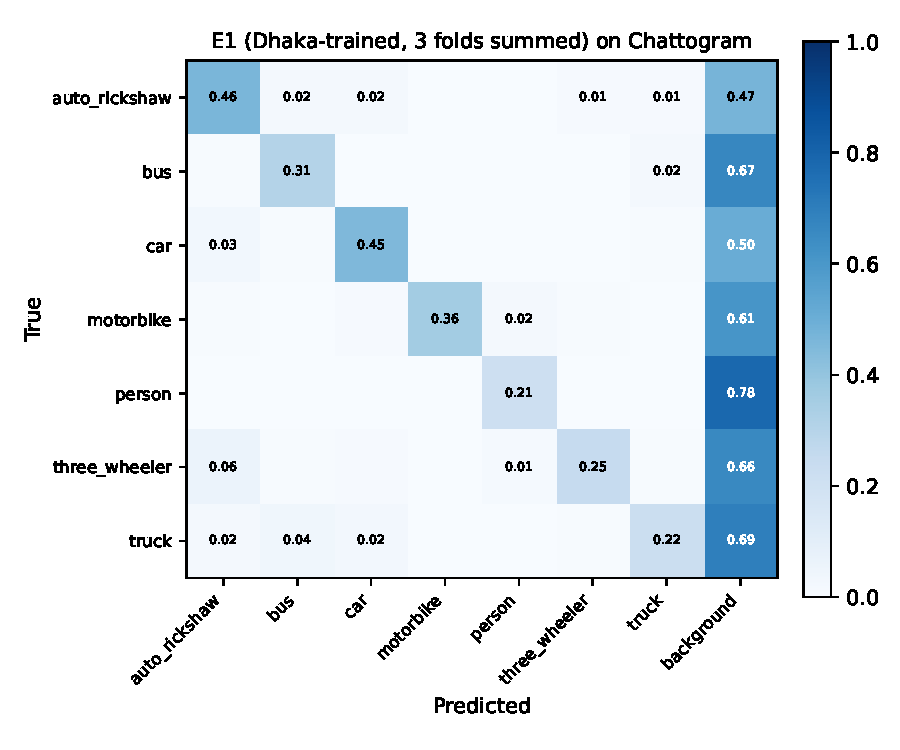
\includegraphics[width=0.44\linewidth]{figures/confusion_e1.pdf}
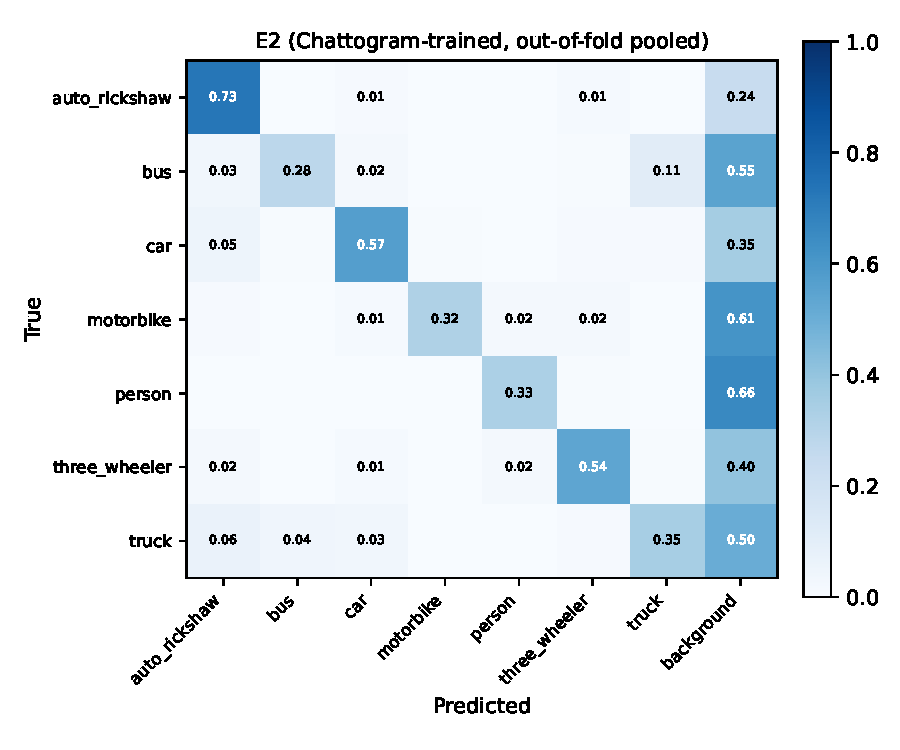
\includegraphics[width=0.44\linewidth]{figures/confusion_e2.pdf}
\caption{Row-normalised confusion matrices (headline classes + background; IoU
$\geq$0.5 greedy match) for E1 (left, 3 Dhaka folds summed) and E2 (right,
Chattogram out-of-fold pooled), both on \texttt{ctg\_pooled\_eval}. A GT box with no
matching prediction counts as ``background'' in that row (a miss); a prediction with
no matching GT counts as ``background'' in that column (a false positive).}
\label{fig:confusion}
\end{figure*}

Figure \ref{fig:confusion} breaks the recall gap down into misses vs.\ misclassifications.
For E1, the background column (missed detections) is the dominant off-diagonal entry
for every headline class, and is visibly larger for \texttt{auto\_rickshaw} and
\texttt{three\_wheeler} than for \texttt{car}/\texttt{person} -- consistent with the
recall-gap ranking in Table \ref{tab:headline}. The largest specific
misclassification in the E1 matrix is \texttt{three\_wheeler} predicted as
\texttt{auto\_rickshaw} under E1 (6\% of true \texttt{three\_wheeler} instances),
plausibly reflecting genuine visual similarity between cycle-rickshaws and motorised
three-wheelers rather than a purely random error -- this confusion is smaller under
E2, suggesting Chattogram-specific visual cues (not present in Dhaka training data)
help separate the two classes.

\subsection{Day/night stratification}
\begin{table}[t]
\centering
\caption{AP50 transfer gap by mode group, stratified by day vs.\ night. Restricted to headline classes only (below-threshold classes not included: non-motorised = \texttt{three\_wheeler} only here, vs.\ + bicycle/cart in Table 2).}
\label{tab:daynight}
\begin{tabular}{lrr}
\toprule
Mode group & Day AP50 gap & Night AP50 gap \\
\midrule
Formal motorised & +0.125 & +0.017 \\
Pedestrian & +0.109 & +0.068 \\
Informal motorised & +0.144 & +0.219 \\
Non-motorised & +0.253 & +0.136 \\
\bottomrule
\end{tabular}
\end{table}

Table \ref{tab:daynight} splits the mode-group AP50 gap by day (456 images) vs.\ night
(665 images), the same day/night proportions reported in \texttt{notes/splits.md}.
The informal-motorised and non-motorised gaps stay large and positive in both
conditions. The formal-motorised gap, however, is not uniformly small: by day it is
+0.125, close to the informal-motorised gap and driven mainly by \texttt{truck} and
\texttt{bus}, while at night it nearly vanishes (+0.017) because \texttt{bus},
\texttt{motorbike} and \texttt{truck} individually reverse sign (E1 outperforming E2).
The pooled formal-motorised number reported earlier therefore averages over two quite
different regimes, and the class concentration of the gap is sharpest at night -- a
day/night interaction worth flagging rather than averaging away.

\subsection{Qualitative failures}
Figure \ref{fig:qualitative} (Section \ref{sec:dataset}) shows the images E1 fails on most severely relative to
E2. Several are low-light, glare-affected frames where E1 detects nothing at all
while E2 recovers every box -- consistent with the day/night finding above, though
the auto-selection was not conditioned on time of day. Because selection is by
recall drop alone, several frames come from the same short sequence
(\texttt{chittagong\_night1}, frames 8520--8580); a de-duplicated selection (e.g.\ one
frame per sequence) is a natural refinement for a later revision.

\subsection{Reverse transfer}
Evaluating the Chattogram-trained models on their corresponding Dhaka fold (a
different direction of transfer) shows every class degrading relative to that fold's
own Dhaka-trained in-domain score, as expected. Here the classes hit hardest are
\texttt{truck} and \texttt{bus} (AP50 dropping by 0.24--0.39), not the informal or
non-motorised classes -- so the class-concentration of the transfer penalty is
direction-dependent, not a fixed per-class difficulty ranking (Section
\ref{sec:discussion}).

\section{Discussion}
\label{sec:discussion}

\subsection{Why this matters beyond detection accuracy}
A detector deployed for automated traffic counting does not report AP50; it reports a
count. A class with lower recall is one whose vehicles are disproportionately missing
from that count. If informal and non-motorised modes are the ones most often missed
when a detector is transferred to a new city without local retraining, any downstream
use of those counts -- e.g.\ converting classified counts to passenger-car-unit
demand for signal-timing allocation -- would systematically under-represent the
travel demand of the road users least able to absorb the resulting delay. This concern
is not hypothetical: Dhaka-specific traffic-signal control work already proposes using
detected vehicle counts directly for congestion-optimised signal timing
\cite{azam2025dhakasignal}, which would make the detection-level blind spot documented
here a direct input to such a pipeline rather than a purely abstract downstream risk.
This paper measures the detection-level premise of that chain; we do not measure the
downstream counting or allocation effect here.

\subsection{Limitations}
The camera viewpoint in both cities is a dash-mounted smartphone, not a fixed traffic
camera of the kind an actual deployed monitoring system would use -- a separate,
already-established axis of domain gap \cite{sharma2026bmd45}, orthogonal to the one
studied here. All data comes from one dataset and one annotation protocol; class
definitions are the dataset authors', not ours. City is not the only variable that
differs between the Dhaka and Chattogram splits -- lighting and road-type mix also
differ. We match day/night ratio and training-set size by construction between the
Dhaka and Chattogram training sets (Section \ref{sec:dataset}), and stratify the
headline result by day/night directly (Table \ref{tab:daynight}) rather than only
controlling for it in aggregate; we do not control for road-type mix. The 4
below-threshold classes cannot support an individual claim at all; they are reported
only in aggregate. Both architectures tested are single-stage Ultralytics YOLO models;
two-stage and transformer-based detectors are untested. The qualitative failure selection (Figure \ref{fig:qualitative})
is unconditioned on sequence identity, so several selected frames come from the same
short video clip rather than being independent samples.

\section{Conclusion}
Holding annotation protocol and camera viewpoint fixed, we find that the
Dhaka-to-Chattogram detection transfer gap is not spread evenly across vehicle classes. It is
smallest for car, bus, truck and motorbike -- classes any general-purpose detector
would already know -- and $3$--$4\times$ larger for two locally-specific informal and
non-motorised modes, auto-rickshaws and cycle-rickshaws, with an even larger gap in
recall specifically. The pattern replicates under an independent leave-one-corridor-out
robustness check and under a newer detector architecture (YOLO26s), which raises
absolute accuracy but leaves the gap essentially unchanged. Because missed vehicles are what would later bias a classified
traffic count, this class-concentrated blind spot is a plausible mechanism for
downstream inequity in any traffic-management system built on a detector transferred
without local retraining -- a link we intend to measure directly in future work.

\bibliographystyle{IEEEtran}
\bibliography{refs}

\end{document}
